\documentclass[10pt,letterpaper,xcolor=dvipsnames,handout]{beamer}

%\usepackage[colorlinks=true,linkcolor=blue]{hyperref}
\usepackage{amssymb,mathabx}
\usepackage{linguex}
\usepackage{verbatim,enumerate,multirow}
\usepackage{xcolor}
%\usepackage{floatflt}

\include{beamer-ru101f14}
\include{tikz-venn-diagrams}

\AtBeginSection[]
{
     \begin{frame}<beamer>
       \frametitle{Lecture plan}
       \tableofcontents[currentsection,currentsubsection]
   \end{frame}
}

\title{Categorical logic 2}
\subtitle{The Aristotelian perspective}
\author[Hoversten]{Erik Hoversten}
\institute[lrp-f14]{Logic, reason, and persuasion: fall 2014 \\ Rutgers University}
\date[10/06/2014]{October 6, 2014}

\begin{document}

\begin{frame}
\titlepage
\end{frame}

\frame{
\frametitle{Boolean perspective}
\framesubtitle{Standard propositions}

\begin{tikzpicture}
  \catvenn{y}{All}{}{}{A}{}{B}
  
  \begin{scope}[shift={(2in,0in)}]
    \catvenn{y}{No}{}{}{C}{}{D}
  \end{scope}
  
  \begin{scope}[shift={(0,-1.5in)}]
    \catvenn{y}{Some}{}{}{E}{}{F}
  
  \begin{scope}[shift={(2in,0in)}]
    \catvenn{y}{Some}{not}{}{G}{}{H}
  \end{scope}
  \end{scope}
\end{tikzpicture}

}

\frame{
\frametitle{Boolean perspective}
\framesubtitle{With complement classes}

\begin{tikzpicture}
  \catvenn{y}{All}{}{non-}{I}{}{J}
  
  \begin{scope}[shift={(2in,0in)}]
    \catvenn{y}{Some}{}{non-}{K}{}{L}
  \end{scope}
  
  \begin{scope}[shift={(0,-1.5in)}]
    \catvenn{y}{Some}{}{non-}{M}{non-}{N}
  
  \begin{scope}[shift={(2in,0in)}]
    \catvenn{y}{No}{}{non-}{O}{}{P}
  \end{scope}
  \end{scope}
\end{tikzpicture}

}

\section{Aristotelian perspective}

\frame{
  \frametitle{Aristotelian perspective}
  \framesubtitle{}
  
  \begin{block}{Existential import}
   \begin{itemize}
    \item In order for universal propositions ($All$, $No$) to be true, there must be at least one member of the subject class.
    \item If the subject class is empty, then the proposition is automatically false.
   \end{itemize}
  \end{block}
  
  \vspace{.75cm}
  
  \uncover<2->{
  \begin{center}
  \begin{tikzpicture}
  \catvenn{y}{All}{}{}{A}{}{B}
  \xmidA
  
  \begin{scope}[shift={(2in,0in)}]
    \catvenn{y}{No}{}{}{C}{}{D}
    \xleftA
  \end{scope}
  \end{tikzpicture}
  \end{center}
  }
}

\frame{
  \frametitle{The traditional square of opposition}
  \framesubtitle{}
 
   \begin{block}{Semantic relations}
   \begin{itemize}
    \item When we take the Aristotelian perspective, we can define more interesting semantic relations between propositions.
    \item Adding these relations to the square of opposition gives us the \textbf{traditional} square of opposition.
   \end{itemize}
  \end{block}
  
  \uncover<2->{
  \begin{center}
   \begin{tikzpicture}
    \sqroppTrad
   \end{tikzpicture}
  \end{center}
  }
}

\frame{
  \frametitle{Semantic relations}
  \framesubtitle{}
  
  \begin{block}<2->{Contradictory}
   \begin{itemize}
    \item The related propositions have opposite truth values.
   \end{itemize}
  \end{block}
  
    \begin{block}<3->{Contrary}
   \begin{itemize}
    \item At least one of the propositions is false (and maybe both are).
   \end{itemize}
  \end{block}
  
    \begin{block}<4->{Subcontrary}
   \begin{itemize}
    \item At least one of the propositions is true (and maybe both are).
   \end{itemize}
  \end{block}
  
    \begin{block}<5->{Subalternation}
   \begin{itemize}
    \item If the top proposition is true, the so is the bottom one (truth flows downward).
    \item If the bottom proposition is false, then so is the top one (falsity flows upward).
   \end{itemize}
  \end{block}
}

\frame{
\frametitle{Contradictory}
\framesubtitle{Opposite truth values}

  \begin{center}
 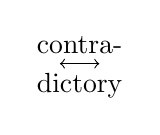
\begin{tikzpicture}
  \catvenn{y}{All}{}{}{A}{}{B}
  \xmiddle
  
  \draw[<->] (3.4cm,0) -- (3.9cm,0) node [above, pos=.5] {contra-} node [below,pos=.5] {dictory};
  \begin{scope}[shift={(6cm,0)}]
    \catvenn{y}{Some}{not}{}{A}{}{B}
  \end{scope}
 \end{tikzpicture}

  \vspace{.75cm}
 
 \uncover<2->{
 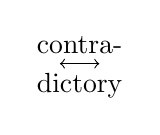
\begin{tikzpicture}
  \catvenn{y}{Some}{}{}{A}{}{B}
  
  \draw[<->] (3.4cm,0) -- (3.9cm,0) node [above, pos=.5] {contra-} node [below,pos=.5] {dictory};
  \begin{scope}[shift={(6cm,0)}]
    \catvenn{y}{No}{}{}{A}{}{B}
    \xleftA
  \end{scope}
 \end{tikzpicture}
 \end{center}
 }
}

\frame{
\frametitle{Contrary}
\framesubtitle{Not both can be true, but both could be false}


  \begin{center}
 \begin{tikzpicture}
  \catvenn{y}{All}{}{}{A}{}{B}
  \xmidA
  
  \draw[<->] (3.4cm,0) -- (3.9cm,0) node [above,pos=.5] {incomp-} node [below,pos=.5] {atible};
  \begin{scope}[shift={(6cm,0)}]
    \catvenn{y}{No}{}{}{A}{}{B}
    \xleftA
  \end{scope}
    \begin{scope}[shift={(0,-3.75cm)}]
    \catvenn{y}{All}{}{}{A}{}{B}
    \xmidA
  \draw[<->] (3.4cm,0) -- (3.9cm,0) node [above, pos=.5] {contra-} node [below,pos=.5] {dictory};
  \begin{scope}[shift={(6,0in)}]
    \catvenn{y}{Some}{not}{}{A}{}{B}
  \end{scope}
  \draw (2cm,-1.25cm) node {False};
  \end{scope}
  \draw[<->] (6.5cm,-1.8cm) -- (6.5cm,-2.2cm) node [right,pos=.5] {compatible};
 \end{tikzpicture}
 \end{center}
}

\frame{
\frametitle{Subcontrary}
\framesubtitle{Not both can be false, but both could be true}


\begin{center}
\begin{tikzpicture}
  \catvenn{y}{Some}{}{}{A}{}{B}
  \draw (2cm,-1.25cm) node {False};
  \draw[<->] (3.4cm,0) -- (3.9cm,0) node [above, pos=.5] {contra-} node [below,pos=.5] {dictory};;
  \begin{scope}[shift={(6cm,0)}]
    \catvenn{y}{No}{}{}{A}{}{B}
    \xleftA  
  \end{scope}
  
  \begin{scope}[shift={(0,-3.75cm)}]
    \catvenn{y}{Some}{not}{}{A}{}{B}
    \draw (2cm,-1.25cm) node {False};
  \draw[<->] (3.4cm,0) -- (3.9cm,0) node [above,pos=.5] {contra-} node [below,pos=.5] {dictory};
  \begin{scope}[shift={(6cm,0)}]
    \catvenn{y}{All}{}{}{A}{}{B}
    \xmidA
  \end{scope}
  \end{scope}
  \draw[<->] (6.5cm,-1.8cm) -- (6.5cm,-2.2cm) node [right,pos=.5] {incompatible};
 \end{tikzpicture}
 \end{center}

}

\frame{
\frametitle{Subalternation}
\framesubtitle{Truth flows down, falsity flows up}


\begin{center}
\begin{tikzpicture}
  \catvenn{y}{All}{}{}{A}{}{B}
  \xmidA
  \draw[->] (0,-1.8cm) -- (0,-2.2cm) node [right, pos=.5] {truth};
  \begin{scope}[shift={(6cm,0)}]
    \catvenn{y}{No}{}{}{A}{}{B}
    \xleftA
    \draw (2cm,-1.25cm) node {False};
  \end{scope}
  %\draw[<->] (3.4cm,0) -- (3.9cm,0) node [above, pos=.5] {contra-} node [below,pos=.5] {dictory};
  \begin{scope}[shift={(0,-3.75cm)}]
    \catvenn{y}{Some}{}{}{A}{}{B}
    %\draw[->] (3.25cm,0) -- (3.75cm,0) node [above, pos=.5] {$false$};
  \begin{scope}[shift={(6cm,0)}]
    \catvenn{y}{Some}{not}{}{A}{}{B}
    \draw (2cm,-1.25cm) node {False};
  \end{scope}
  \end{scope}
  %\draw[<->] (3.8cm,-2.1cm) -- (3.3cm,-1.7cm) node [above=.25cm,pos=.5] {$contra$};
  %\draw[<->] (3.3cm,-2.1cm) -- (3.8cm,-1.7cm) node [right,pos=.5] {};
    \draw[<-] (6.5cm,-1.8cm) -- (6.5cm,-2.2cm) node [right,pos=.5] {falsity};
 \end{tikzpicture}
 \end{center}

}

\section{Validity}

\frame{
\frametitle{Validity}
\framesubtitle{Premiese are at least as strong as the conclusion}

 \begin{itemize}
  \item<+-> A categorical argument is valid if the conclusion doesn't say anything that the premises don't also say.
  \item<+-> An argument is invalid if either:
    \begin{itemize}
     \item The conclusion contradicts something said by a premise
     \item The conclusion says something that isn't said by a premise
    \end{itemize}
   \item<+-> Conditional validity:
     \begin{itemize}
  \item If all we know is a universal, then we don't actually know if the subject class has any members.
  \item We say that an argument involving a universal term is \textbf{conditionally valid} if it would be valid so long as the subject term has members.
 \end{itemize}
 \end{itemize}


\begin{block}<4->{``What is said by a proposition''}
\small
 \begin{itemize}
  \item We can use Venn diagrams to visualize what a proposition says.
  \item Every mark (shading or x) in the diagram is something ``said'' by the proposition.
 \end{itemize}
\end{block}


}

\frame{
\frametitle{Validity}
\framesubtitle{Examples}

 \begin{center}
 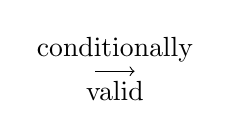
\begin{tikzpicture}
  \catvenn{y}{All}{}{}{A}{}{B}
  \xmidA
  
  \draw[->] (3.4cm,0) -- (3.9cm,0) node [above, pos=.5] {conditionally} node [below,pos=.5] {valid};
  \begin{scope}[shift={(6cm,0)}]
    \catvenn{y}{Some}{}{}{A}{}{B}
  \end{scope}
 \end{tikzpicture}

  \vspace{.75cm}

 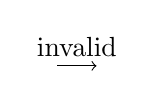
\begin{tikzpicture}
  \catvenn{y}{Some}{}{}{A}{}{B}
  
  \draw[->] (3.4cm,0) -- (3.9cm,0) node [above, pos=.5] {invalid};
  \begin{scope}[shift={(6cm,0)}]
    \catvenn{y}{All}{}{}{A}{}{B}
    \xmidA
  \end{scope}
 \end{tikzpicture}
 \end{center}

}

\frame{
\frametitle{Evaluating inferences}
\framesubtitle{}

\begin{block}{Translate sentences}
 \begin{itemize}
  \item The semantic relations we looked at allow us to infer the truth value of a proposition from the truth value of a different proposition.
  \item So, if an argument says that one proposition is false, we know that there is a different proposition that will be true.
  \item This allows us to get all of the propositions in the argument into standard form.
 \end{itemize}
\end{block}

\begin{block}<2->{Compare the diagrams}
 \begin{itemize}
  \item Once all the propositions are in standard form, we can use the associated Venn diagrams to compare what each proposition says.
  \item If the diagram for the conclusion has no more and no different marking than the diagram for the premise, then the argument is valid.
 \end{itemize}

\end{block}

}

\frame{
\frametitle{Example}
\framesubtitle{All A are B.  Therefore, it is false that no A are B.}

\begin{center}
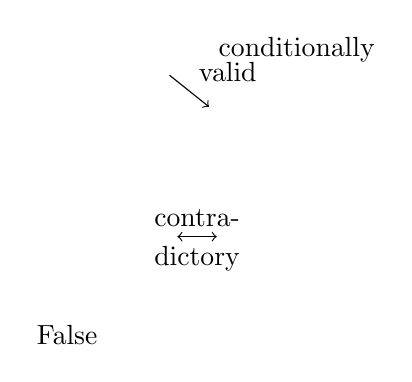
\begin{tikzpicture}
  \catvenn{y}{All}{}{}{A}{}{B}
  \xmidA
  %\draw[->] (0,-1.8cm) -- (0,-2.2cm) node [right, pos=.5] {};
  
  %\draw[->] (3.25cm,0) -- (3.75cm,0) node [above, pos=.5] {$contra$};
  \begin{scope}[shift={(0,-3.75cm)}]
    \catvenn{y}{No}{}{}{A}{}{B}
    \xleftA
    \draw (2cm,-1.25cm) node {False};
    \draw[<->] (3.4cm,0) -- (3.9cm,0) node [above, pos=.5] {contra-} node [below,pos=.5] {dictory};
  \begin{scope}[shift={(6cm,0)}]
    \catvenn{y}{Some}{}{}{A}{}{B}
  \end{scope}
  \end{scope}
  \draw[<-] (3.8cm,-2.1cm) -- (3.3cm,-1.7cm) node [above right,pos=.5] {valid} node [above right=.25cm,pos=.5] {conditionally};
  %\draw[<->] (3.3cm,-2.1cm) -- (3.8cm,-1.7cm) node [right,pos=.5] {};
   % \draw[<-] (6.5cm,-1.8cm) -- (6.5cm,-2.2cm) node [right,pos=.5] {};
 \end{tikzpicture}
 \end{center}


}


\frame{
\frametitle{Next meeting}
\framesubtitle{}

\begin{block}{What's coming up?}
 \begin{itemize}
  \item More on categorical syllogisms: proving validity
  \item Read Ch. 5
  \item HW\#2 will be returned in class
 \end{itemize}

\end{block}

}

\end{document}